\section{Building Models on Human Perception}
\label{sec:models}

The previous section has yielded interesting results from human labelling (Section \ref{sec:human}). We concluded that a temporal dimension, and a lexical compensator might help in improving existing FER models for speaking subjects. 

Our current FER models are working on static images, which means that we will have to temporalize them in some way. We will discuss this in section \ref{sub:temp}. A lexical compensator will have to be done with a separate model. There are different approaches to this, as we have seen in section \ref{sec:existing}. We will discuss this in section \ref{sub:lex}.


\subsection{Temporal Dimension}
\label{sub:temp}
As discussed previously, we want to keep and build on existing FER models. Given that some of our models will work on video data, we will have to temporalize our models which currently work on static images.

The straight forward approach is to take the current model, and wrap it in a temporal layer. This means that an input video with 60 frames will produce 60 output embeddings, which can then be fed into a recurrent layer like a LSTM or GRU. This produces minimal overhead, while preserving all weights from our model.

We will use this approach in all our upcoming models.

To have a comparison between frame sizes and an estimation of the importance of the temporal dimension, our models were trained on 1, 30, 60, and 90 frames.

\begin{figure}
    \centering
    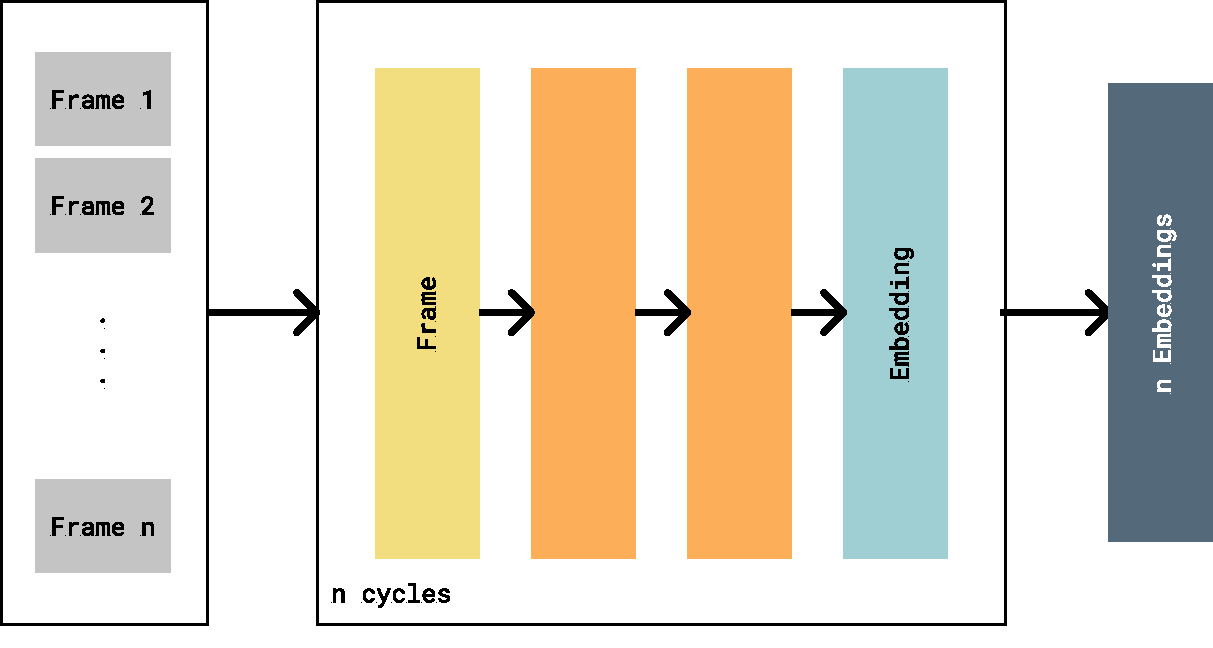
\includegraphics[width=0.8\textwidth]{res/temporalization.pdf}
    \caption{Temporalizing an FER model. The existing model gets wrapped in a TimeDimensional layer. That way the model produces $n$ embeddings for $n$ inputs.}
    \label{fig:temporalization}
\end{figure}

\subsection{Lexical Compensators}
\label{sub:lex}
Lexical compensators can come in different shapes and forms. We will focus on the two previously mentioned approaches from Bursic \cite{bursic2020improving} and Busso \cite{salman2020style}, which attempt to extract lexical information in different ways.

\paragraph{LipNet} 
Bursic et al. \cite{bursic2020improving} used a LipNet embedding to detect the lexical content. We reproduced their approach to analyse the performance of the architecture, using our own MobileNet. The dataset of choice, similarly to the original model, was RAVDESS. The validation data consisted of all the recordings of actors 4, 5, 9, and 14.

\paragraph{Style Extractor}
The lexical compensator of Salman and Busso \cite{salman2020style} served as the inspiration for our own. However, we made some changes to the architecture and preprocessing of the style extractor. We turned to FaceMesh as a facial landmark detector, yielding 468 three-dimensional coordinates, 1404 inputs in total. We chose a smaller, non temporal architecture network, with only one hidden layer.

We trained several different models to optimize the size of the style extractor. Given that a hidden layer of 3000 neurons overtrained the model, we drastically stepped down to 512, 256, and 128 neurons. The validation loss of the model was chosen as the deciding metric. 
All three smaller models generalized well with a very similar validation loss. We ultimately continued with the smallest models, yielding a more compact model.

Another difference to the original approach was our decision to remove the second, unused output which predicts the underlying phoneme. Several test runs using a phoneme output yielded no improvement on the actual style extractor output.

The dataset used to train this model, like in the original paper, was CREMA-D.

\begin{figure}
    \centering
    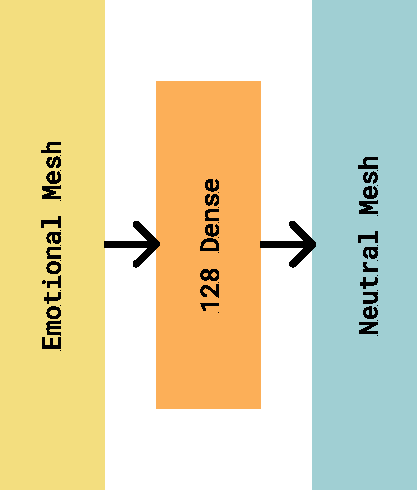
\includegraphics[width=0.5\textwidth]{res/FExtractor.pdf}
    \caption{The architecture of our final feature extractor. The emotional input mesh of a subject speaking a given phoneme $p$ gets passed to a densely connected hidden layer with 128 neurons. The output of the network is a prediction of a neutral mesh of the actor pronouncing the same phoneme $p$.}
    \label{fig:fextractor}
\end{figure}

\subsection{Building the Models}

To complete the architecture, we will breifly talk about the the fusion layers. In instances where two model inputs come together (e.g. the lexical compensators) we need a network that combines both inputs. We want this fusion network to be consistent across all our models to make sure that differences in results are not due to differing architectures.

We turned to the fusion layer by Bursic et al. \cite{bursic2020improving}. We already try to replicate their approach with the lexical compensation from LipNet, and our FER model has a similar embedding with 512 neurons to their VGG19 model. This lets us better compare our results to theirs. In comparison to the model from Salman and Busso \cite{salman2020style}, this fusion network covers all seven core emotions.

To judge the impact of the lexical compensators we also trained a model that only uses the temporalized embedding of our FER model. We use the same fusion network, this time in a transfer learning approach. The FER embedding of 512 neurons gets passed to the same fusion network, foregoing the \texttt{concatenate} step. This aides in comparing the impact of the lexical compensators without having any noise from a differing transfer network.

The input from the previous model(s) are fed into a bidirectional GRU layer of size 256. A dense layer of size 16 follows. The final output layer is a densely connected layer of size 7, corresponding to the core emotions. The activation function of the hidden layers are ReLU, while the output layer has a softmax activation function. A dropout layer of 0.5 is placed between the GRU and the following dense layer (see Figure \ref{fig:fusionlayers}).

We end up with three main architectures:

\begin{enumerate}
    \item \textbf{Temporal FER model} The temporalized FER model without a lexical compensator.
    \item \textbf{Lexical compensation with LipNet} The temporalized FER model with LipNet as the lexical compensator.
    \item \textbf{Lexical compensation with our style extractor} The temporalized FER model with a self trained style extractor as the lexical compensator.
\end{enumerate}

\begin{figure}
    \centering
    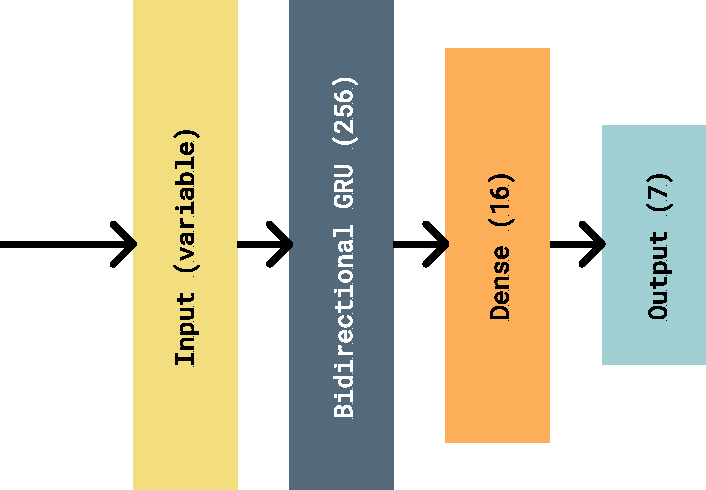
\includegraphics[width=0.7\textwidth]{res/FusionLayers.pdf}
    \caption{The architecture of the fusion/transfer network. It is kept simple to accommodate the smaller datasets we use and follows the architecture from Bursic et al. \cite{bursic2020improving}.}
    \label{fig:fusionlayers}
\end{figure}
\subsection{Data and Preprocessing}
\paragraph{Data for FER Models}
We mainly use two datasets in our work, RAVDESS and CREMA-D. Since the actual usage of the data is dependent on some preprocessing steps like face-/mouth-cropping and landmark extraction, we transformed the datasets before starting the training cycles on them.

The FER-model takes a facial crop of the frame, with 224x224x3 dimensions (width, height, colour channels). In preprocessing, we saved a crop of every frame for all videos. 
The LipNet model needs a 100x50x3 dimensional input of the orofacial area. This crop is saved alongside the facial crop for each frame. Both the facial and orofacial crops were done with the frontal face detector of dlib \cite{dlib09}.

Finally, our lexical compensator will be trained on facial landmarks extracted from FaceMesh. Those are also stored with the facial and orofacial crops.

Each videos data is saved as an array in a \texttt{pickle} file. The structure of the file can be seen in figure \ref{fig:pickle}.
\begin{figure}
    \centering
    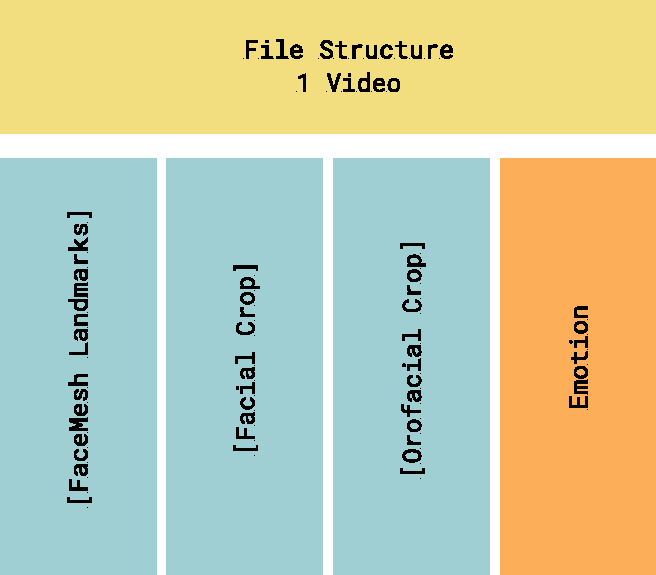
\includegraphics[width=0.5\textwidth]{res/Pickle.pdf}
    \caption{The data structure of our preprocessed files. Each file corresponds to one video. Its facial and orofacial crops, alongside with its facial landmarks are stored in arrays. The array lengths correspond to the amount of frames in each video. The underlying emotion is saved as well.}
    \label{fig:pickle}
\end{figure}

\paragraph{Data for the Style Extractor}
To be able to train the style extractor we need pairs of meshes for every phoneme, where one mesh was emotional (not neutral) and one neutral. To have a more fine-grained model, we also wanted to make sure that all mesh pairs are from the same occurrence. As an example, the sentence "It's eleven \textbf{o}'cl\textbf{o}ck" has two occurrences of the phoneme \texttt{O} (marked). When training the style extractor, all mesh pairs came from the same actor in the same sentence at similar positions.


\subsection{Training}
Here we present some more detailed information for the training process of our models.
\paragraph{General Information}
To keep the models comparable on the temporal dimension, we trained each model on 1, 30, 60, and 90 frames. The FER and LipNet model were pre-trained and locked. We wanted to cover the core emotions that were defined by Ekman, and thus ignored the \texttt{calm} emotion that was provided by the RAVDESS dataset.

To get the most out of each video, we used a sliding window approach on the frame arrays. Given a model with a frame size of 60 and a video with 100 frames, we now have the opportunity to extract multiple data point from the video. We used a window stride of 5. This means that the first data point ranges from frame 0 to 59, the second from 5 to 64 and so on. This helped to somewhat ease the problem of the RAVDESS dataset being too small for proper DNN training. 

Our specific feature extractor was trained separately. It was trained on CREMA-D, with actors 1 to 11 being used for validation.

The fusion networks for all models was trained on RAVDESS. Actors 4, 5, 9, and 14 were used for the validation set, the files from the other 20 actors were used for training.

\paragraph{Technical Details}
We used the \texttt{keras} environment using a \texttt{tensorflow} backend (version 2.4.1) to train our models on a HPC using an Nvidia Titan X GPU with the Pascal architecture. The scripts were deployed in Docker containers, on a server running Ubuntu 18.04 LTS.

\subsection{Results}
In this chapter we will present the results of our training. More detailed results and discussion can be found in section \ref{sec:discussion}.
